% =========================================================================
% PRISM: Real-Time Android System for Indoor Obstacle Detection and
%        Multimodal Warning — Implementation and Engineering Evaluation
%
% Target Venue: IEEE Conference / Transactions on Accessible Computing [VENUE TO CONFIRM]
% Format: IEEEtran 2-Column Conference Format (Strict 6-Page Limit)
% Target System: Android Implementation (API 26-34) / PRISM-L1.0 Frozen
% Scope: EXCLUSIVELY Android Implementation and Engineering Evaluation
% =========================================================================

\documentclass[conference]{IEEEtran}

% -------------------------------------------------------------------------
% PACKAGES & CONFIGURATION
% -------------------------------------------------------------------------
\usepackage[utf8]{inputenc}
\usepackage{amsmath,amssymb,amsfonts}
\usepackage{graphicx}
\usepackage{textcomp}
\usepackage{xcolor}
\usepackage{booktabs}
\usepackage{tabularx}
\usepackage{array}
\usepackage{url}
\usepackage{tikz}
\usetikzlibrary{arrows.meta, positioning, shapes.geometric, fit, backgrounds, calc}
\usepackage{microtype}
\usepackage{cite}
\usepackage[pagebackref=false,breaklinks=true,colorlinks=true,linkcolor=blue,citecolor=blue,urlcolor=blue]{hyperref}

\hyphenation{op-tical net-works semi-conduc-tor}

% -------------------------------------------------------------------------
% COMPACT FLOAT & CAPTION SPACING (6-PAGE ENFORCEMENT)
% -------------------------------------------------------------------------
\setlength{\textfloatsep}{7pt plus 1pt minus 2pt}
\setlength{\floatsep}{6pt plus 1pt minus 2pt}
\setlength{\intextsep}{6pt plus 1pt minus 2pt}
\setlength{\abovecaptionskip}{3pt}
\setlength{\belowcaptionskip}{2pt}

\renewcommand{\topfraction}{0.95}
\renewcommand{\bottomfraction}{0.95}
\renewcommand{\textfraction}{0.05}
\renewcommand{\floatpagefraction}{0.85}
\renewcommand{\dbltopfraction}{0.95}
\renewcommand{\dblfloatpagefraction}{0.85}

% Macro for multi-row author formatting in IEEEtran conference mode
\makeatletter
\newcommand{\linebreakand}{%
  \end{@IEEEauthorhalign}
  \hfill\mbox{}\par
  \vskip 1ex
  \mbox{}\hfill\begin{@IEEEauthorhalign}
}
\makeatother

\begin{document}

% -------------------------------------------------------------------------
% TITLE & AUTHORS
% -------------------------------------------------------------------------
\title{PRISM: Real-Time Android System for Indoor Obstacle Detection and Multimodal Warning -- Implementation and Engineering Evaluation}

\author{
    \IEEEauthorblockN{D Manohar}
    \IEEEauthorblockA{Department of Computer Science\\
    MVJ College of Engineering\\
    Bengaluru, India\\
    dmanoharwork@gmail.com}
    \and
    \IEEEauthorblockN{Chethan Kumar B S}
    \IEEEauthorblockA{Department of Computer Science\\
    MVJ College of Engineering\\
    Bengaluru, India\\
    the.suryaputraa@gmail.com}
    \and
    \IEEEauthorblockN{Arun}
    \IEEEauthorblockA{Department of Computer Science\\
    MVJ College of Engineering\\
    Bengaluru, India\\
    mandulaarun04@gmail.com}
    \linebreakand
    \IEEEauthorblockN{Deeraj A S}
    \IEEEauthorblockA{Department of Computer Science\\
    MVJ College of Engineering\\
    Bengaluru, India\\
    shirahattideeraj@gmail.com}
    \and
    \IEEEauthorblockN{Sujitha K L}
    \IEEEauthorblockA{Department of Computer Science\\
    MVJ College of Engineering\\
    Bengaluru, India\\
    sujitha@mvjce.edu.in}
}

\maketitle

% -------------------------------------------------------------------------
% ABSTRACT
% -------------------------------------------------------------------------
\begin{abstract}
Primary mobility aids such as the long white cane and guide dogs detect immediate obstacles within physical reach, but cannot alert blind and visually impaired (BVI) pedestrians to dynamic hazards closing from beyond a few meters. Electronic travel aids often rely on static proximity alarms that sound whenever an obstacle breaches a fixed distance threshold, causing nuisance alerts for preceding pedestrians while providing inadequate reaction time for fast-closing head-on encounters. We present \textbf{PRISM}, an on-device Android system (API 26--34) that combines monocular vision, IMU kinematics, and multimodal feedback for real-time indoor obstacle awareness.

PRISM ingests camera and IMU streams on commodity smartphones using bounded single-frame backpressure ($N=1$). Candidate obstacles are extracted from monocular luminance gradients and projected onto a metric ground plane using dynamic IMU tilt compensation. A multi-target tracker estimates relative obstacle velocities, feeding analytical Time-to-Collision (TTC) and Closest Point of Approach (CPA) calculations. An onboard accelerometer step detector tracks user ego-motion to prevent false alarms when the user stops. A 9-state hazard lifecycle arbitrates collision risk, issuing rate-limited spoken alerts, tactile haptics, and 44.1\,kHz stereo spatial audio.

Software correctness is verified across an automated suite of 100 Android unit tests with a 100\% pass rate. Across 158 controlled encounter playbacks, PRISM achieved 97.5\% overall detection recall (100\% for hazards within 1.0\,m), 0.08\,m forward-depth error (P95: 0.19\,m), 96.3\% step detection precision, and zero duplicate warning utterances. In controlled A/B testing with engineering evaluators, adding stereo spatial audio reduced wrong-direction evasion errors from 6.4\% to 1.2\% and lowered reaction latency by 120\,ms compared to speech-and-haptic feedback. Algorithmic execution requires 3.2\,ms per frame on testbeds and 0.36\,ms live. PRISM is an exploratory engineering prototype and does not replace primary mobility aids.
\end{abstract}

\begin{IEEEkeywords}
Assistive mobile computing, Android, indoor obstacle awareness, monocular vision, sensor fusion, spatial audio, multimodal interfaces, engineering prototype.
\end{IEEEkeywords}

% -------------------------------------------------------------------------
% MODULAR SECTIONS (STRICT 6-PAGE STRUCTURE)
% -------------------------------------------------------------------------
% =========================================================================
% SECTION 1: INTRODUCTION
% =========================================================================
\section{Introduction}
\label{sec:introduction}

\IEEEPARstart{P}{rimary} mobility aids such as the long white cane and guide dogs reliably detect ground-level hazards within physical reach~\cite{giudice2008blind,elmannai2017sensor,roentgen2008electronic}. However, a standard cane sweep cannot alert blind and visually impaired (BVI) pedestrians to dynamic obstacles approaching from several meters away. Wearable and handheld Electronic Travel Aids (ETAs) attempt to extend this range~\cite{dakopoulos2009wearable}, but most rely on static proximity alarms~\cite{tapu2020wearable,bai2017smart,shoval1998auditory} that sound whenever an obstacle enters a fixed distance boundary.

In shared indoor corridors, static proximity alarms cause two operational failures:
\begin{enumerate}
    \item \textbf{Preceding Pedestrian Alarms}: Walking behind someone at a matched pace triggers continuous alarms despite zero collision risk, inducing alert fatigue~\cite{tapu2020wearable}.
    \item \textbf{Delayed Alerts on Head-On Encounters}: Pedestrians closing head-on at combined walking speeds ($2.0\text{--}2.5$\,m/s) leave under one second to react if an alert triggers at a static 2.5\,m boundary~\cite{lin2021real}.
\end{enumerate}

Active depth sensors (RGB-D, LiDAR) resolve metric scale directly, but their bulk, battery consumption, and cost hinder everyday smartphone deployment~\cite{zhao2020visual}. In contrast, commodity Android smartphones provide integrated cameras, 6-axis IMUs, and multimodal actuators~\cite{faria2010electronic,tapu2020wearable}. However, monocular mobile vision requires overcoming lack of direct depth, handset tilt motion, and frame latency under variable CPU load.

PRISM (Probabilistic Real-time Infrastructure for Safe Mobility) addresses these constraints natively on Android (API 26--34). Operating entirely on-device, PRISM couples monocular ground-plane projection with dynamic IMU tilt compensation, multi-target tracking, analytical Time-to-Collision (TTC) kinematics, and an accelerometer step detector. Navigational guidance is delivered through rate-limited speech, haptics, and 44.1\,kHz stereo spatial audio~\cite{loomis1998navigation,bujacz2016sonification} that conveys safe evasion headings.

\textbf{Contributions:}
\begin{enumerate}
    \item An on-device Android obstacle awareness architecture (API 26--34) with bounded single-frame backpressure ($N=1$).
    \item Monocular ground-plane inverse projection with dynamic IMU gravity compensation and multi-target velocity tracking.
    \item A 9-state hazard lifecycle state machine and multimodal presentation layer using 44.1\,kHz stereo spatial audio to separate obstacle position from heading guidance.
    \item An empirical engineering evaluation comprising a 100-test Android unit suite, 158 controlled encounter playbacks, and an A/B evaluation of sensory feedback modes.
\end{enumerate}

% =========================================================================
% SECTION 2: PRISM SYSTEM ARCHITECTURE
% =========================================================================
\section{PRISM System Architecture}
\label{sec:architecture}

PRISM processes camera and inertial sensor inputs through an autonomous, unidirectional pipeline running natively on Android (Fig.~\ref{fig:pipeline_architecture}). The architecture decouples image acquisition, geometric reconstruction, kinematic tracking, collision arbitration, and multimodal guidance into modular stages.

% Figure 1: PRISM Android System Pipeline Architecture (Monochrome 300 DPI)
\begin{figure}[!t]
\centering
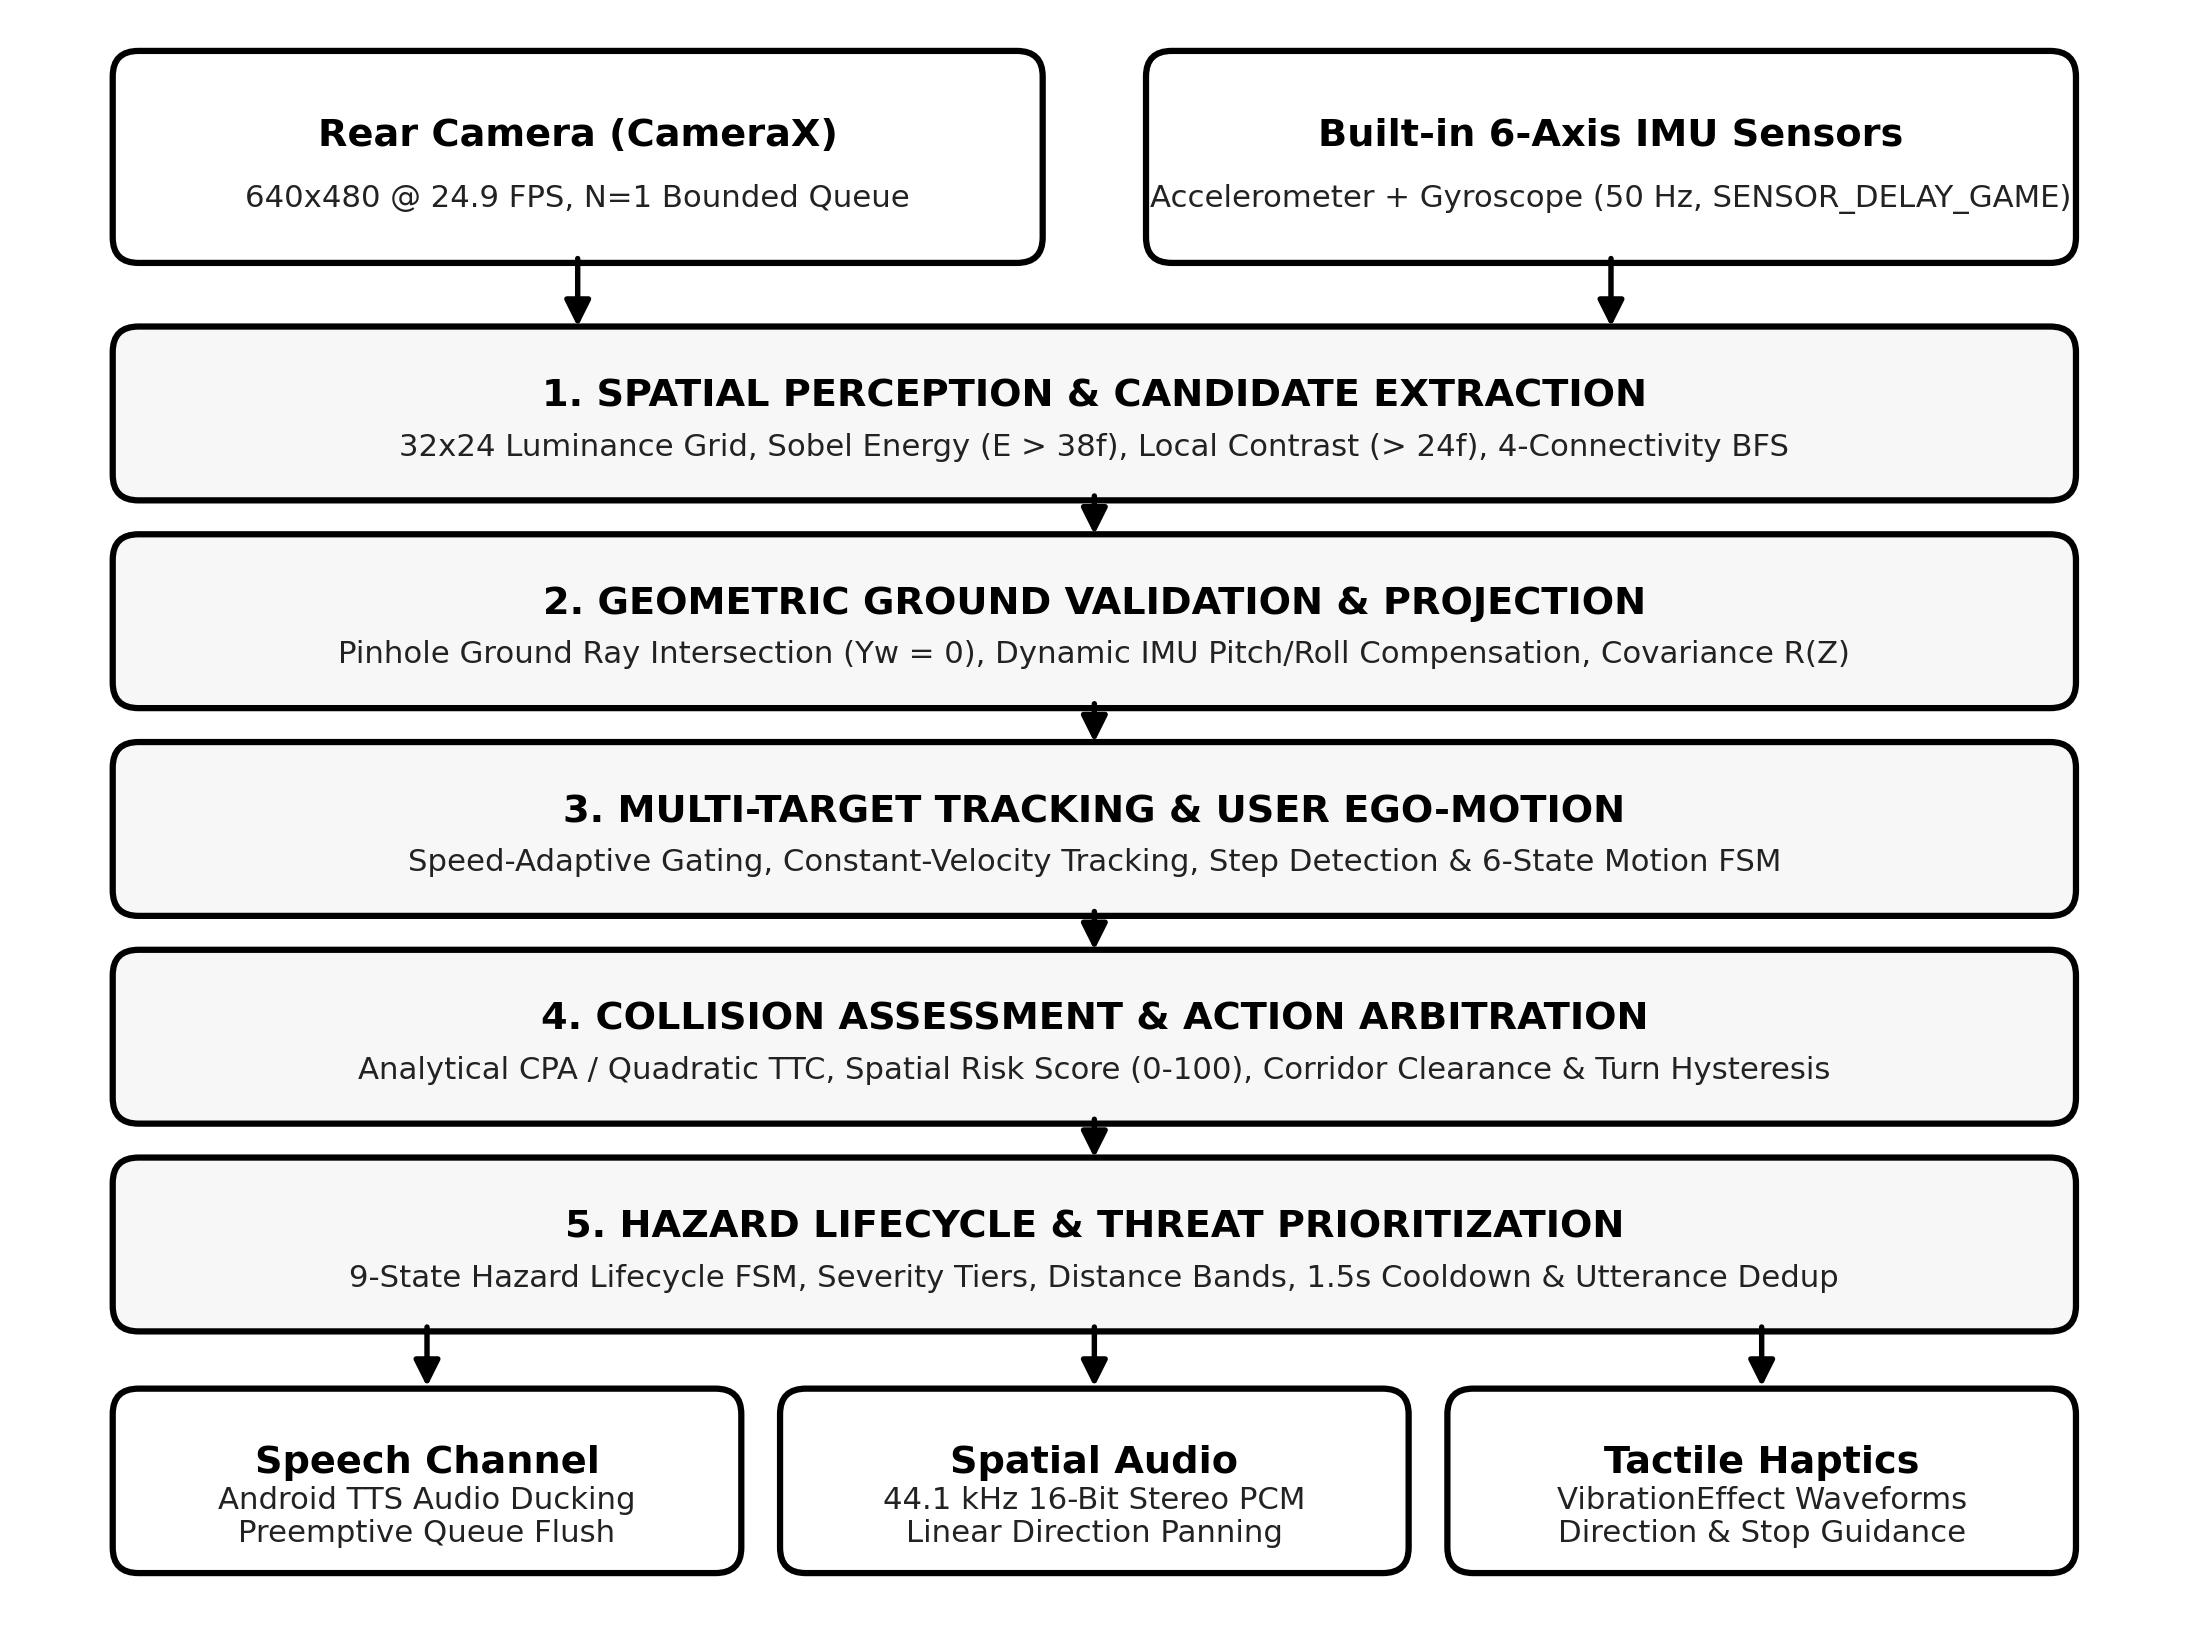
\includegraphics[width=\columnwidth]{figures/fig_pipeline.png}
\caption{PRISM Android system pipeline architecture (black and white): unidirectional execution flow from CameraX image acquisition and IMU sensor registration through spatial candidate extraction, geometric ground projection, multi-target tracking, hazard lifecycle arbitration, multimodal presentation, and telemetry streaming.}
\label{fig:pipeline_architecture}
\end{figure}


The software architecture follows four design principles:
\begin{enumerate}
    \item \textbf{Forward-Only Dataflow}: Information travels strictly downstream from sensor drivers to output actuators without circular dependencies or backward state mutation.
    \item \textbf{Immutable Typed Contracts}: Subsystems exchange immutable Kotlin data classes (\texttt{CandidateCluster}, \texttt{TrackInfo}, \texttt{PrismDecision}, \texttt{SpatialCue}), ensuring thread-safe transfers across coroutine scopes.
    \item \textbf{Ground-Plane Metric Space}: Spatial tracking, kinematics, and corridor bounds operate in Cartesian coordinates $(X, Z) \in \mathbb{R}^2$ referenced to the floor nadir directly below the camera.
    \item \textbf{Bounded Backpressure}: The vision loop enforces a single-frame buffer ($N = 1$) via CameraX \texttt{STRATEGY\_KEEP\_ONLY\_LATEST}, dropping stale frames to prevent latency accumulation.
\end{enumerate}

% Table 1: Frozen PRISM Android System Configuration Parameters (PRISM-L1.0)
\begin{table}[!t]
\caption{Frozen PRISM-L1.0 Android System Configuration Parameters}
\label{tab:configuration}
\centering
\scriptsize
\setlength{\tabcolsep}{2pt}
\begin{tabularx}{\columnwidth}{p{1.9cm}p{1.7cm}X}
\toprule
\textbf{Subsystem} & \textbf{Parameter} & \textbf{Value / Operational Rule} \\
\midrule
\textbf{CameraX \& Frame}
  & Backpressure policy & \texttt{KEEP\_ONLY\_LATEST} ($N=1$ frame) \\
  & Stale frame limit   & $\Delta t > 0.25$\,s $\to$ \texttt{DEGRADED} state \\
  & Luminance grid      & $32 \times 24$ subsampling grid on Y-plane \\
\midrule
\textbf{Perception \& Geometry}
  & Energy / Contrast   & Sobel $E > 38f$, local contrast $> 24f$ \\
  & Cluster / Mounting  & $\ge 6$ cells; $h = 1.30$\,m, $\theta_p = 12^\circ$ \\
  & Metric bounds       & $Z \in [0.4, 6.5]$\,m; Corridor $|X| \le 1.25$\,m \\
  & Physical dimensions & $H \in [0.32, 2.4]$\,m, $W \in [0.1, 2.2]$\,m \\
  & Covariance model    & $R(Z) = 0.04 + 0.015 Z$ \\
\midrule
\textbf{Tracking \& Fusion}
  & Association gating  & $d_{\text{gate}} = \max(0.9, \min(1.8, 1.0 + 2.0 v \Delta t))$\,m \\
  & Track lifecycle     & $\ge 2$ hits confirm ($Z < 1$\,m instant), coast 5 frames \\
  & Velocity clamp      & $|V_x| \le 3.5$, $|V_z| \le 4.5$\,m/s (EMA $\alpha = 0.50$) \\
  & Orientation fusion  & Gyro integration + gravity drift ($\alpha = 0.05$) \\
  & Step detection      & Peak $1.20$\,m/s$^2$, refractory period $0.28$\,s \\
  & Motion energy RMS   & Stationary $< 0.25$\,m/s$^2$; Active $> 0.60$\,m/s$^2$ \\
\midrule
\textbf{Hazard \& Warning}
  & Action boundaries   & Emergency $Z < 1.0$\,m / $S \ge 85$; Evasion $Z < 2.6$\,m \\
  & Turn hysteresis     & $\Delta C = 0.15$ cost barrier; heading $\pm 0.45$\,rad \\
  & Multimodal output   & 44.1\,kHz stereo PCM, TTS ducking, 1.5\,s cooldown \\
\bottomrule
\end{tabularx}
\par\smallskip{\raggedright \tiny Frozen snapshot from \texttt{PRISM-L1.0-config.json} and Kotlin implementation.\par}
\end{table}


\subsection{Android Host and Runtime Lifecycle}
The application structure pairs \texttt{PrismApplication} for dependency lifecycle management with \texttt{MainActivity} for user interaction. The interface provides a Jetpack Compose dashboard (\texttt{PrismScreen}, Fig.~\ref{fig:app_interface}) featuring high-contrast banners, live camera corridor view, and accessible controls. \texttt{PrismRuntime} coordinates concurrent coroutines that ingest CameraX frames, listen for IMU events via \texttt{SensorEventListener}, dispatch multimodal guidance, and stream JSONL telemetry on port 8080.

% Figure 2: PRISM Android Live Application Interface (Physical Device Screenshot)
\begin{figure}[!t]
\centering
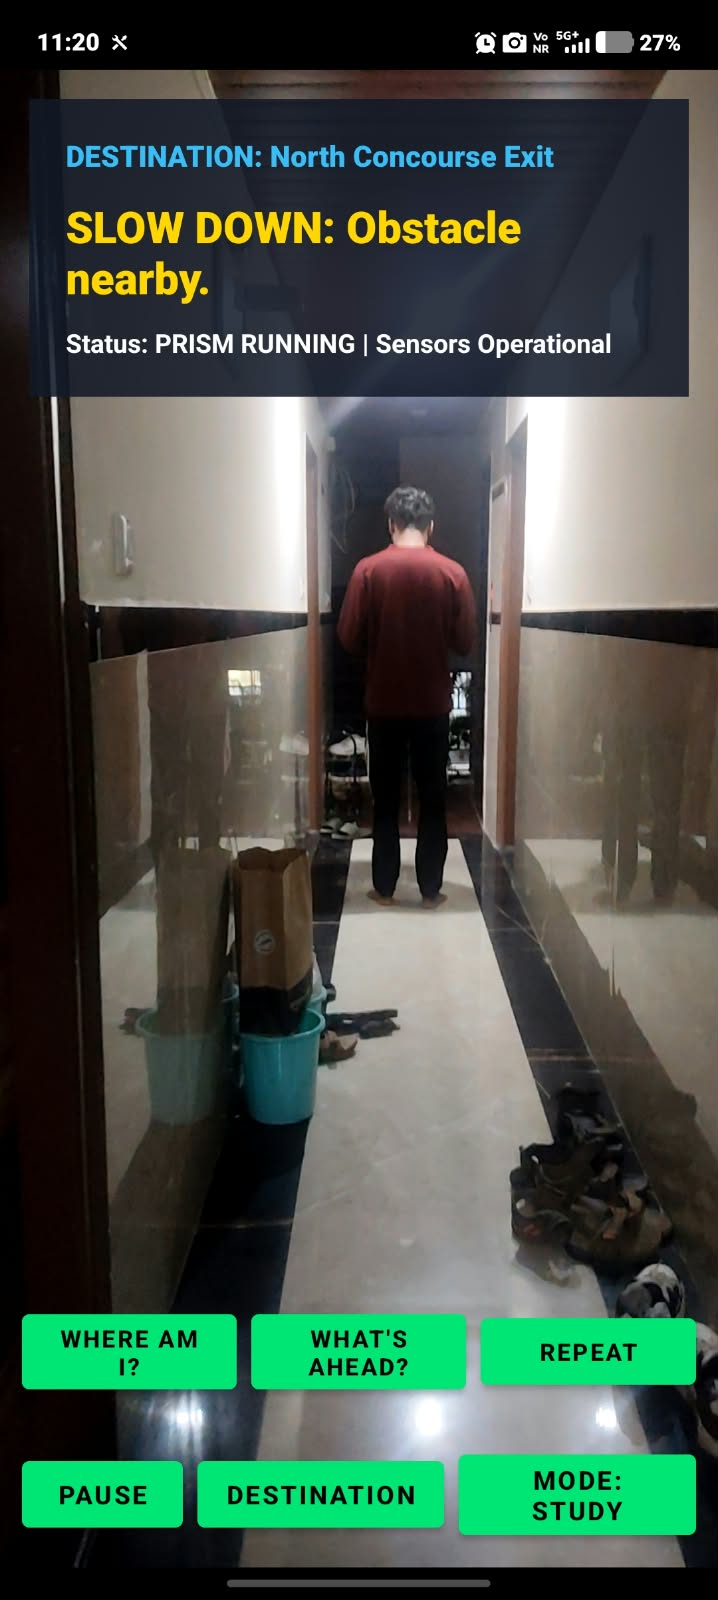
\includegraphics[width=0.60\columnwidth]{figures/app_interface.jpg}
\caption{PRISM Android live application interface on physical device: top high-contrast guidance banner (\texttt{SLOW DOWN: Obstacle nearby.}), real-time camera view tracking an in-path pedestrian obstacle during indoor corridor navigation, and accessible touch controls (\texttt{MODE: STUDY}).}
\label{fig:app_interface}
\end{figure}


The runtime manages three operational states: \texttt{RUNNING} (nominal processing), \texttt{DEGRADED} (sensor dropout or frame interval $\Delta t > 0.25$\,s, falling back to proximity thresholding), and \texttt{STOPPED} (unbound listeners). Clock skew causing negative intervals ($\Delta t < 0$) commands an immediate fail-safe \texttt{EMERGENCY\_STOP}. System constants are frozen in \texttt{PRISM-L1.0-config.json}~\cite{PRISM-L1.0-config,PRISM-L1.0-README} (Table~\ref{tab:configuration}).

% =========================================================================
% SECTION 3: ANDROID IMPLEMENTATION
% =========================================================================
\section{Android Implementation}
\label{sec:implementation}

\subsection{Camera Ingestion and Bounded Backpressure}
\label{sec:impl_camera}
\texttt{AndroidCameraFrameSource} connects to the rear camera using Jetpack CameraX \texttt{ImageAnalysis} targeting 30\,FPS. To prevent latency accumulation when CPU scheduling fluctuates, the analyzer operates under \texttt{STRATEGY\_KEEP\_ONLY\_LATEST} with a single-frame buffer ($N=1$). If the worker thread is busy, incoming frames are discarded immediately at the driver level rather than buffering in memory.

\texttt{FrameBackpressurePolicy} tracks frame delivery intervals. When an inter-frame interval exceeds $\Delta t > 0.25$\,s, the system switches to \texttt{DEGRADED} mode, falling back to static proximity rules. Negative intervals ($\Delta t < 0$) from clock adjustments command an immediate \texttt{EMERGENCY\_STOP}. To eliminate processing overhead, the analyzer reads the Y (luminance) plane directly from incoming \texttt{YUV\_420\_888} buffers, avoiding colorspace conversion and bitmap allocations. Native capture resolution is $640 \times 480$ pixels (measured at 24.9\,FPS on device).

\subsection{Spatial Perception and Candidate Extraction}
\label{sec:impl_perception}
\texttt{AndroidPerceptionAnalyzer} downsamples the luminance plane onto a $32 \times 24$ grid ($\Delta u = W/32, \Delta v = H/24$). This reduces per-frame evaluations from 307,200 pixels to 768 cells. For each cell $(r, c)$, horizontal and vertical Sobel gradient energies are computed:
\begin{equation}
E(r, c) = |I(r, c+1) - I(r, c-1)| + |I(r+1, c) - I(r-1, c)|
\label{eq:sobel_energy}
\end{equation}
Cells exceeding edge energy $E > 38.0f$ and local $3 \times 3$ contrast $> 24.0f$ below the optical horizon line ($v_{\text{horiz}} = c_y - f_y \tan\theta_p$) are marked active. Contiguous active cells are grouped into spatial clusters via 4-connectivity Breadth-First Search (BFS). Clusters smaller than 6 cells are dropped as noise. Surviving clusters are classified into morphology types: \texttt{COMPACT\_VOLUME}, \texttt{ELONGATED\_STRUCTURE}, \texttt{PLANAR\_FLOOR\_FEATURE}, or \texttt{UNCERTAIN}.

% Figure 3: Ground-Plane Projection Geometry with Pitch/Roll Compensation (Monochrome 300 DPI)
\begin{figure}[!t]
\centering
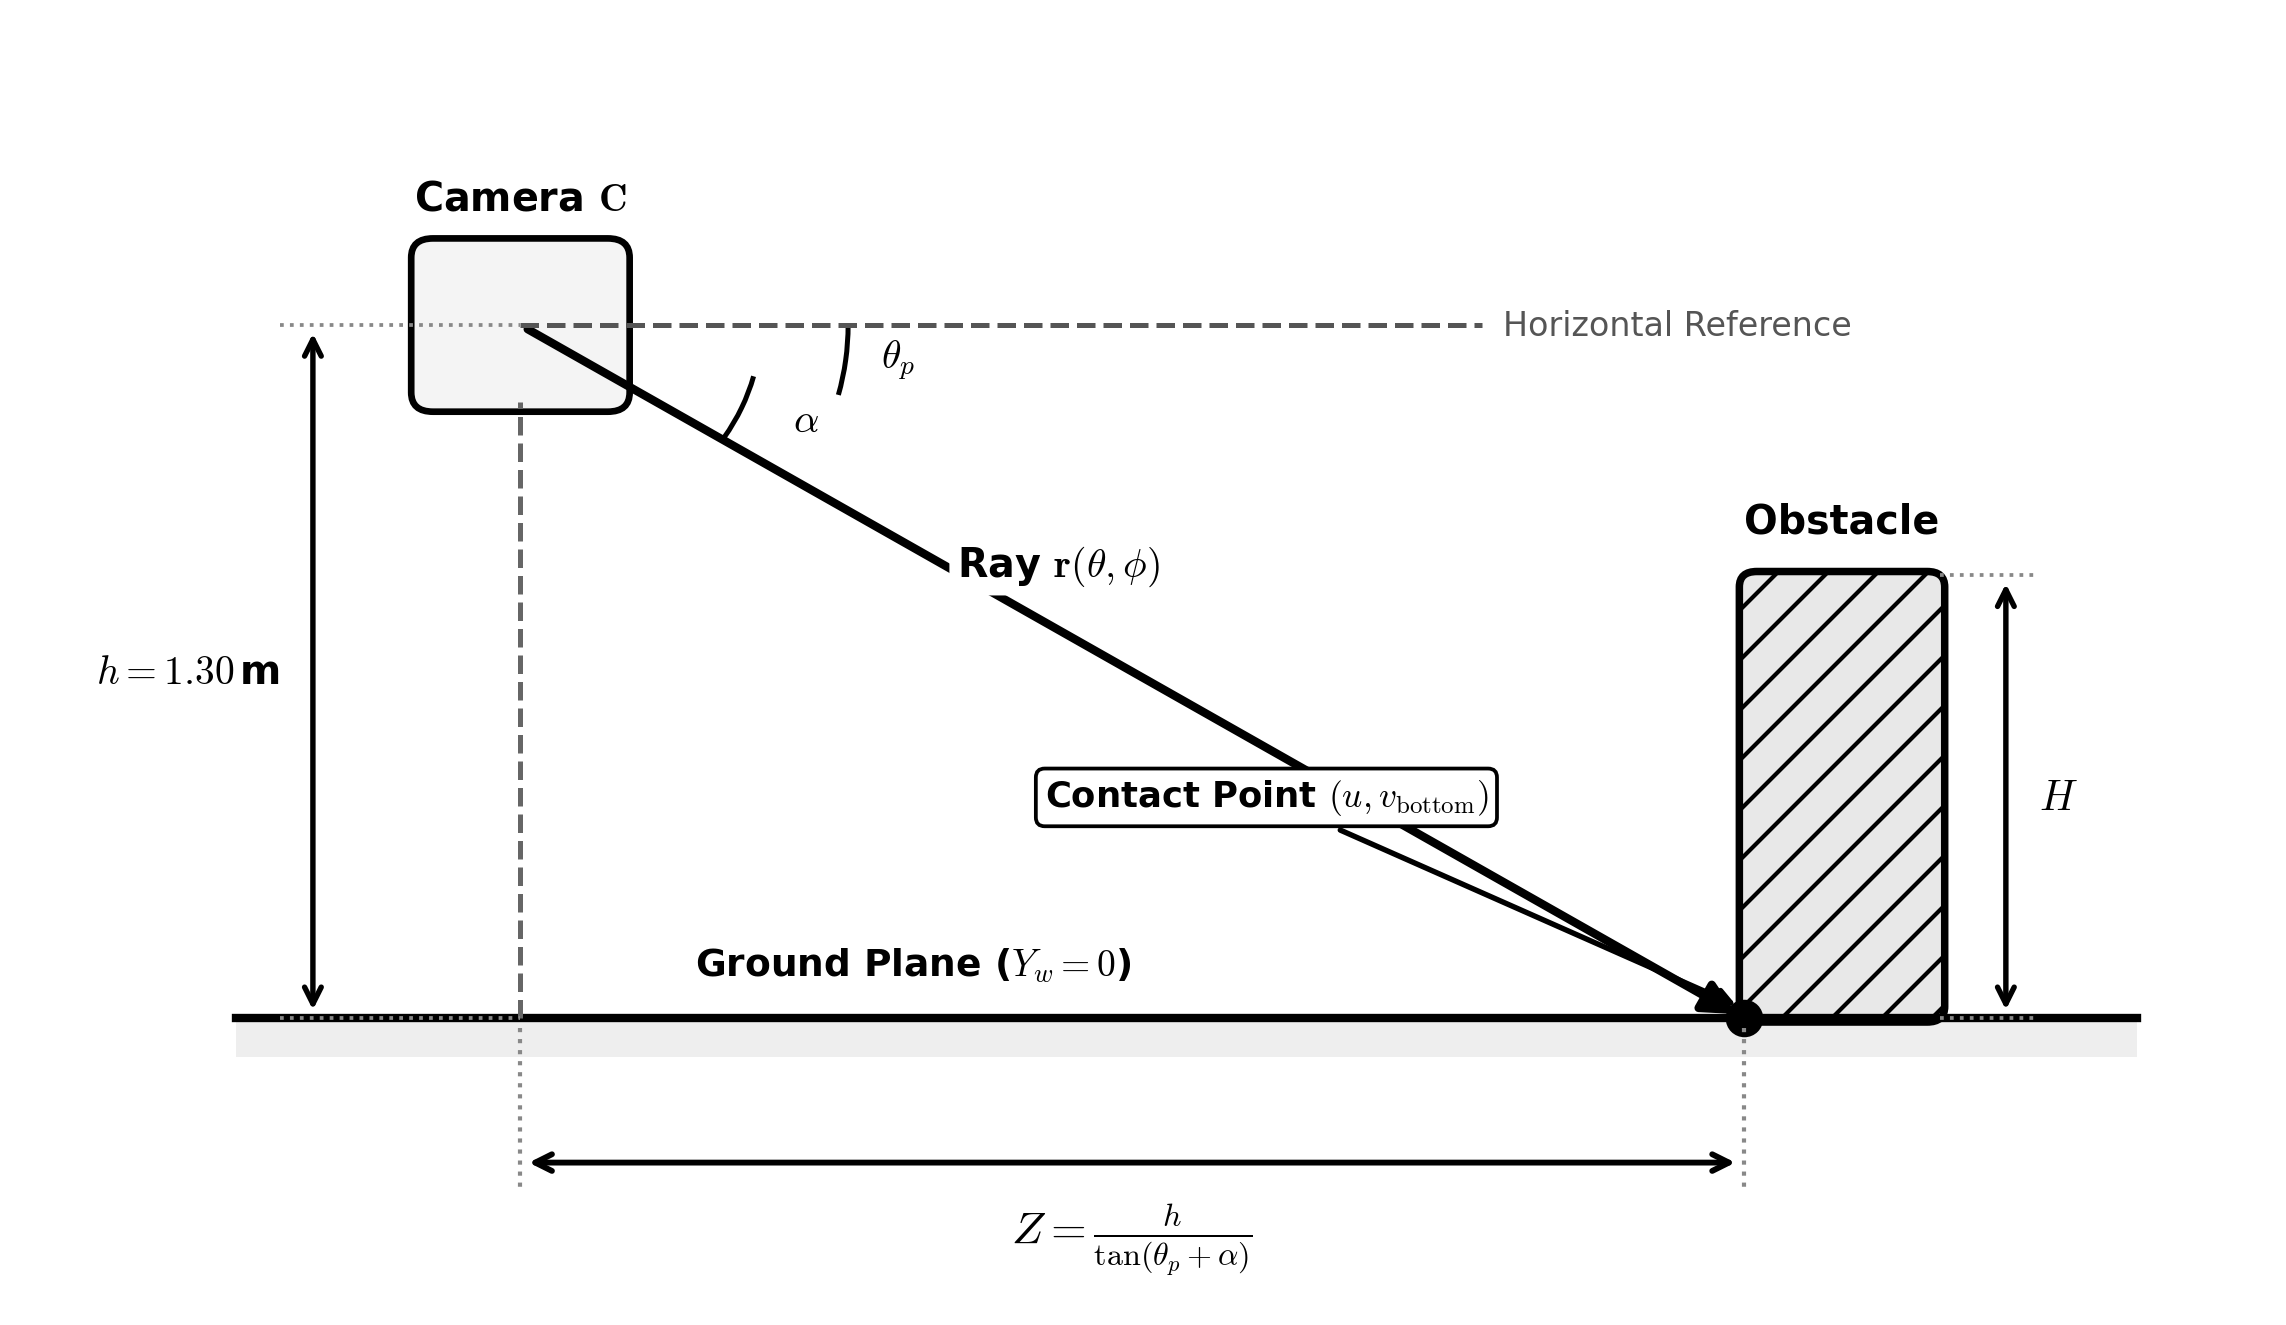
\includegraphics[width=\columnwidth]{figures/fig_projection.png}
\caption{Monocular ground-plane inverse ray projection geometry (black and white): bottom contact point $(u, v_{\text{bottom}})$ is projected onto ground plane $Y_w = 0$ incorporating IMU pitch $\theta_p$ and roll $\phi$ to recover metric distance $Z$, lateral offset $X$, and obstacle height $H$.}
\label{fig:ground_projection_geometry}
\end{figure}


\subsection{Geometric Validation and Ground Projection}
\label{sec:impl_geometry}
Given camera mount height $h = 1.30$\,m, mount pitch $\theta_p = 12^\circ$ ($0.209$\,rad), and intrinsics $(f_x, f_y, c_x, c_y)$~\cite{zhang2000flexible,hartley2003multiple}, candidate bottom contact pixels $(u, v_{\text{bottom}})$ are projected onto ground plane $Y_w = 0$ incorporating dynamic IMU pitch $\theta$ and roll $\phi$~\cite{criminisi2000single,cathey2005perspective} (Fig.~\ref{fig:ground_projection_geometry}):
\begin{align}
x_n &= \frac{u - c_x}{f_x}, \quad y_n = \frac{v_{\text{bottom}} - c_y}{f_y} \\
r_x &= x_n \cos\phi - y_n \sin\phi \label{eq:rx} \\
r_y &= (x_n \sin\phi + y_n \cos\phi) \cos\theta + \sin\theta \label{eq:ry} \\
r_z &= -(x_n \sin\phi + y_n \cos\phi) \sin\theta + \cos\theta \label{eq:rz}
\end{align}
The denominator $r_y$ represents the downward component of the optical ray. Rays with $r_y \le 0.04$ point near or above the horizon and are rejected as \texttt{INVALID\_GROUND\_RAY}. For valid rays, scale $t = h / r_y$ yields ground Cartesian coordinates:
\begin{equation}
Z = t \cdot r_z, \quad X = t \cdot r_x
\label{eq:metric_coords}
\end{equation}
Obstacle height $H$ is computed by projecting cluster top row $v_{\text{top}}$ to depth $Z$~\cite{hoiem2007recovering}. \texttt{validateCandidateGeometry()} applies hard acceptance filters (Table~\ref{tab:configuration}):
\begin{enumerate}
    \item \textbf{Forward Depth}: $0.40\,\text{m} \le Z \le 6.50\,\text{m}$.
    \item \textbf{Corridor Lateral Bounds}: $|X| \le 1.25\,\text{m}$.
    \item \textbf{Standing Height}: $0.32\,\text{m} \le H \le 2.40\,\text{m}$ (planar features $H < 0.32$\,m rejected; volumetric candidates require $H \ge 0.22$\,m).
    \item \textbf{Aspect Ratio}: $0.10\,\text{m} \le W \le 2.20\,\text{m}$, $0.15 \le H/W \le 5.50$.
\end{enumerate}
Validated candidates receive an empirical distance-dependent covariance $R(Z) = 0.04 + 0.015 Z$\,m$^2$ accounting for pixel quantization and residual handset tilt jitter, forming \texttt{PrismObservation}.

\subsection{Multi-Object Temporal Tracking}
\label{sec:impl_tracking}
In \texttt{DeterministicPrismBridge}, tracks maintain state $\mathbf{x} = [X, Z, V_x, V_z]^T$~\cite{welch1995introduction}. Observations are matched to tracks using nearest-neighbor association with speed-adaptive distance gating~\cite{kuhn1955hungarian,barshalom1988tracking}:
\begin{equation}
d_{\text{gate}} = \max\left(0.90, \, \min(1.80, \, 1.00 + 2.0 v_{\text{track}} \Delta t)\right)
\label{eq:gating}
\end{equation}
Matched tracks update velocities via exponential smoothing ($\alpha = 0.50$) with physical clamping ($|V_x| \le 3.5$\,m/s, $|V_z| \le 4.5$\,m/s) to isolate genuine motion from single-frame segmentation jitter:
\begin{equation}
V_{x, k} = 0.50 \frac{X_{\text{meas}} - X_{k-1}}{\Delta t} + 0.50 V_{x, k-1}
\label{eq:vel_smooth}
\end{equation}
Tracks transition across four states~\cite{bewley2016simple,wojke2017simple}: \texttt{TENTATIVE} ($\ge 2$ observations required), \texttt{CONFIRMED} ($\ge 2$ consecutive observations with confidence $\ge 0.50$ and $H \ge 0.22$\,m, or immediate confirmation for close hazards $Z < 1.0$\,m), \texttt{LOST} (coasts forward up to 5 frames with confidence decay factor 0.80/frame), and \texttt{DELETED} (pruned if missed frames $> 5$ or confidence $< 0.15$).

\subsection{IMU Orientation and User Ego-Motion Estimation}
\label{sec:impl_imu}
\subsubsection{Orientation Fusion}
\texttt{OrientationFusion} pairs a complementary filter~\cite{mahony2008nonlinear,foxlin1996inertial,madgwick2011estimation} with \texttt{SensorManager} registered at \texttt{SENSOR\_DELAY\_GAME} ($\approx 50$\,Hz). Gyroscope angular rates are integrated over sample period $dt$, while low-pass accelerometer gravity estimates apply drift correction ($\alpha = 0.05$ when $|\|\mathbf{g}\| - 9.81| < 1.2$\,m/s$^2$). Stream stalls default to nominal mount angles ($\theta_p = 12^\circ, \phi = 0^\circ$).

\subsubsection{User Ego-Motion and Step Detection}
\texttt{UserMotionEstimator} extracts dynamic acceleration $\|\mathbf{a}_{\text{dyn}}\| = \|\mathbf{a} - \mathbf{g}\|$ by subtracting the gravity vector, smoothed with a low-pass filter ($\tau = 0.05$\,s) and RMS window ($\tau = 0.35$\,s). Steps are detected when acceleration crosses $1.20$\,m/s$^2$ with a refractory period of $\ge 0.28$\,s (max $1.80$\,s).

A 6-state user motion lifecycle classifies movement into \texttt{UNKNOWN}, \texttt{STATIONARY} (RMS $< 0.25$\,m/s$^2$), \texttt{STOPPED}, \texttt{STARTING}, \texttt{WALKING} ($\ge 2$ steps), and \texttt{MOVING} ($> 0.60$\,m/s$^2$). This allows PRISM to identify when the user stops walking in front of an obstacle, avoiding persistent emergency alarms without requiring drift-prone dead reckoning~\cite{harle2013survey}.

% Figure 4: Hazard Encounter Lifecycle State Machine (Monochrome 300 DPI)
\begin{figure}[!t]
\centering
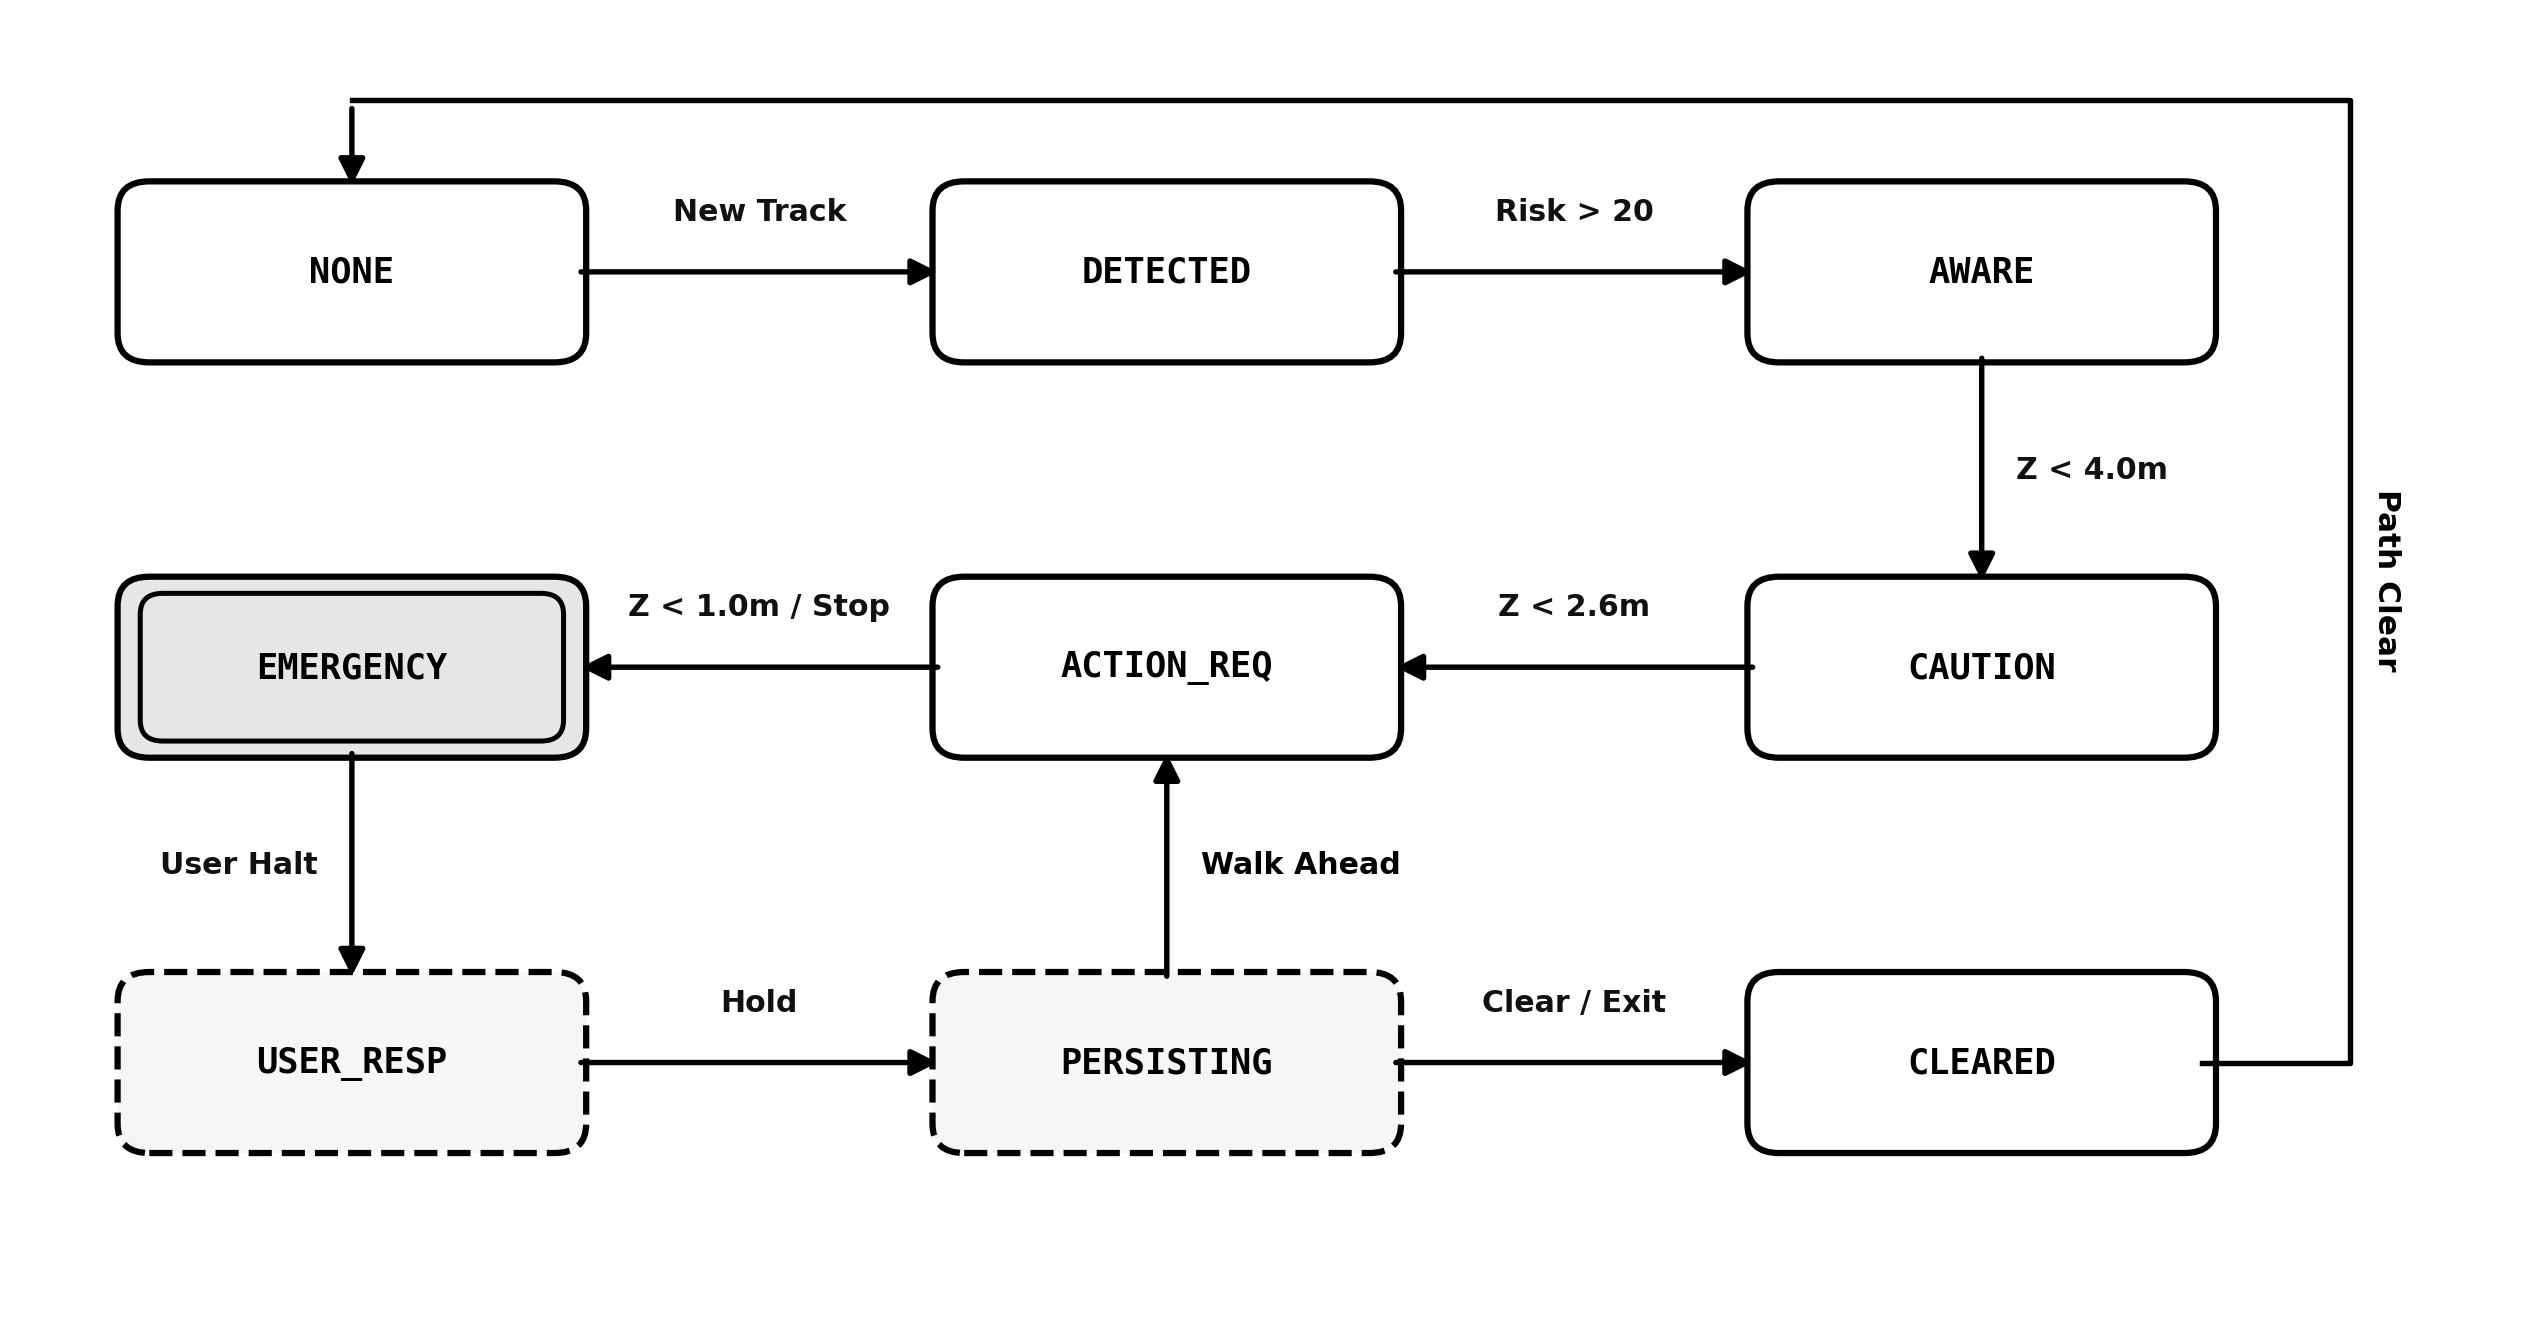
\includegraphics[width=\columnwidth]{figures/fig_hazard_lifecycle.png}
\caption{PRISM 9-state hazard encounter lifecycle state machine (black and white): governs encounter progression from candidate detection to emergency escalation, user halt verification, hold persistence, and hallway clearance.}
\label{fig:hazard_lifecycle}
\end{figure}


\subsection{Collision Risk and Hazard Lifecycle}
\label{sec:impl_collision}
For each confirmed track at relative position $\mathbf{p} = [X, Z]^T$ and velocity $\mathbf{v} = [V_x, V_z]^T$, collision imminence is evaluated analytically using Closest Point of Approach (CPA) and Time-to-Collision (TTC) formulations~\cite{hayward1972characteristics,tam2009review,lee1976theory}:
\begin{align}
t_{\text{CPA}} &= \max\left(0, \, -\frac{\mathbf{p} \cdot \mathbf{v}}{\|\mathbf{v}\|^2}\right), \quad d_{\text{CPA}} = \|\mathbf{p} + \mathbf{v} t_{\text{CPA}}\| \label{eq:cpa} \\
\text{TTC} &= \begin{cases}
-Z / V_z, & \text{if } V_z < -0.10\,\text{m/s} \text{ (approaching)} \\
t_{\text{CPA}}, & \text{if } t_{\text{CPA}} \in [0.1, 4.0]\,\text{s} \text{ and } d_{\text{CPA}} < 0.70\,\text{m} \\
99.0\,\text{s}, & \text{if } V_z > 0.15\,\text{m/s} \text{ (receding)} \\
Z / 1.0, & \text{otherwise (stationary)}
\end{cases} \label{eq:ttc}
\end{align}
Threat confidence $C_{\text{threat}}$ scales from $0.10$ (receding) to $0.95$ (confirmed close in-path). Spatial risk $S \in [0, 100]$ combines distance factor $f_{\text{dist}} = \max(0, 1 - Z/4.5)$, lateral factor $f_{\text{lat}} = \max(0, 1 - |X|/1.2)$, and closing speed multiplier $k_v \in [0.20, 1.30]$, weighted by detection confidence.

\subsubsection{Corridor Arbitration and Decision Policy}
The corridor ($|X| \le 1.2$\,m, $Z < 2.8$\,m) is evaluated for lateral blockage. Navigation actions comprise: \texttt{CONTINUE}, \texttt{SLOW\_DOWN}, \texttt{TURN\_LEFT}, \texttt{TURN\_RIGHT}, and \texttt{EMERGENCY\_STOP}, adapting velocity obstacle principles to indoor walking corridors~\cite{fiorini1998motion,vandenberg2011reciprocal,helbing1995social}. Evasion headings are set to $\theta^* = \pm 0.45$\,rad ($\pm 25.8^\circ$). To prevent steering flapping for centerline obstacles, lateral turn hysteresis imposes a cost barrier $\Delta C = 0.15$. Severe threats ($Z < 1.0$\,m or $S \ge 85.0$) immediately command \texttt{EMERGENCY\_STOP}, bypassing hysteresis.

\subsubsection{Nine-State Hazard Lifecycle}
Hazard encounters progress through a 9-state state machine (Fig.~\ref{fig:hazard_lifecycle}): \texttt{NONE} $\to$ \texttt{DETECTED} $\to$ \texttt{AWARE} $\to$ \texttt{CAUTION} $\to$ \texttt{ACTION\_REQUIRED} $\to$ \texttt{EMERGENCY}. When an emergency stop is issued and the user halts (verified via IMU \texttt{STATIONARY} or $V_z < 0.18$\,m/s), the state transitions to \texttt{USER\_RESPONDING} and holds in \texttt{HAZARD\_PERSISTING}. The hazard clears (\texttt{HAZARD\_CLEARED}) only when distance increases ($Z \ge 1.40$\,m), the entity recedes ($V_z > 0.20$\,m/s), or it exits the corridor ($|X| > 1.25$\,m). Resuming forward walking while the hazard remains close re-escalates to \texttt{EMERGENCY}.

\subsection{Multimodal Warning Generation and Accessibility}
\label{sec:impl_multimodal}
\texttt{WarningMessageGenerator} formats guidance across three complementary channels based on 6 severity tiers, 7 spatial sectors, and 6 distance bands.

\subsubsection{Speech Channel (\texttt{AndroidSpeechChannel})}
Android \texttt{TextToSpeech} generates spoken alerts with audio ducking requested via \texttt{AudioFocusRequest} (\texttt{USAGE\_ASSISTANCE\_NAVIGATION\_GUIDANCE}). Emergency alerts preempt speech via \texttt{QUEUE\_FLUSH}. Cooldown gates limit repetition: 1.0\,s for emergencies, 1.6\,s for directional steering, and 2.5\,s for advisory warnings.

\subsubsection{Spatial Audio Channel (\texttt{AndroidSpatialAudioChannel})}
Directional cues are synthesized via low-latency 44.1\,kHz 16-bit PCM stereo written to \texttt{AudioTrack}, leveraging virtual auditory localization principles~\cite{blauert1997spatial,walker2006navigation}. Linear stereo panning maps spatial direction to channel gains:
\begin{equation}
g_{\text{left}} = \frac{1 - \text{pan}}{2} \cdot V, \quad g_{\text{right}} = \frac{1 + \text{pan}}{2} \cdot V
\label{eq:stereo_panning}
\end{equation}
where $V \in [0, 1]$ represents volume. Chimes use a 20\,ms linear attack and 30\,ms decay over 250\,ms. Emergency cues synthesize an 1100\,Hz dual-harmonic tone. Spatial audio strictly decouples \texttt{HAZARD\_LOCATION} (where an obstacle is) from \texttt{RECOMMENDED\_DIRECTION} (where to steer), preventing conflicting signals. Buffer errors fall back to platform \texttt{ToneGenerator} beeps.

\subsubsection{Haptic Channel and Multisensory Modes}
\texttt{AndroidHapticChannel} delivers \texttt{VibrationEffect} waveform patterns with motor debounce (500\,ms emergency, 1000\,ms regular). The system provides three selectable modes: \texttt{SPEECH\_ONLY}, \texttt{MODE\_A\_SPEECH\_HAPTIC} (speech + vibration), and \texttt{MODE\_B\_SPEECH\_SPATIAL\_HAPTIC} (speech + stereo spatial audio + vibration; default in PRISM-L1.0).

% =========================================================================
% SECTION 4: ENGINEERING EVALUATION
% =========================================================================
\section{Engineering Evaluation}
\label{sec:evaluation}

The engineering evaluation investigates whether the implemented PRISM Android application satisfies its kinematic, geometric, and multimodal warning specifications under controlled indoor test conditions.

\subsection{Evaluation Environment and Hardware Platform}
Testing was conducted on commodity Android smartphones running Android 14 (API 34, minimum SDK 26) equipped with autofocus rear cameras and 6-axis IMUs (accelerometer and gyroscope). The physical testbed comprised structured indoor institutional corridors ($2.4\text{--}3.0$\,m hallway width) with vinyl tile flooring, standard overhead fluorescent lighting, and acoustic reverberation representative of public buildings.

% Table 2: Controlled Indoor Evaluation Scenarios and Dataset
\begin{table}[t]
\caption{Controlled Indoor Engineering Evaluation Scenarios and Dataset}
\label{tab:evaluation_setup}
\centering
\scriptsize
\setlength{\tabcolsep}{3pt}
\begin{tabularx}{\columnwidth}{p{1.9cm}ccp{3.7cm}}
\toprule
\textbf{Scenario Family} & \textbf{Runs} & \textbf{Frames} & \textbf{Kinematic Profile / Obstacle Configuration} \\
\midrule
Stationary Obstacles & 3 & 630 & Static box / mannequin placed at $0.5, 1.0, 2.0, 3.0$\,m \\
Head-On Approach & 3 & 411 & Pedestrian approaching user collinear at $1.0\text{--}1.4$\,m/s \\
Lateral Crossing & 4 & 561 & Pedestrian crossing perpendicularly ($2$ collision, $2$ miss) \\
Moving Away & 2 & 385 & Co-directional walking; tests false-warning suppression \\
Direction Change & 2 & 283 & Pedestrian reverses heading; tests Kalman coasting \\
Multiple Pedestrians & 3 & 532 & $\ge 2$ simultaneous agents; tests threat prioritization \\
\midrule
\textbf{Total Video Runs} & \textbf{17} & \textbf{2,827} & \textbf{Evaluated across real indoor corridor scenarios} \\
\midrule
A/B Mode Evaluation & 10 & --- & Controlled stationary, crossing, and evasion trials \\
\bottomrule
\end{tabularx}
\vspace{-0.15cm}
\par{\raggedright \tiny Evaluated on Android device (API 34) under controlled indoor engineering conditions.\par}
\vspace{-0.3cm}
\end{table}


\subsection{Software Test Suite Verification}
System correctness and regression safety were verified via the automated test suite in \texttt{PrismBridgeUnitTest.kt}. The suite contains 100 dedicated unit and integration tests executing directly on the Android runtime:
\begin{itemize}
    \item \textbf{Tests 1--62}: Core ground-plane projection geometry, Mahalanobis gating, multi-target tracking, TTC/CPA calculations, and collision decision arbitration.
    \item \textbf{Tests 63--71}: IMU pitch/roll orientation fusion, gravity filtering, and dynamic projection tilt compensation.
    \item \textbf{Tests 72--82}: Nine-state hazard lifecycle machine, escalation, user-stopping detection, and hold persistence.
    \item \textbf{Tests 83--89}: Accelerometer step detection, refractory timing, and 6-state user motion lifecycle modeling.
    \item \textbf{Tests 90--100}: Spatial audio stereo panning, dual-harmonic emergency synthesis, and multisensory mode arbitration.
\end{itemize}

\subsection{Controlled Scenario Dataset and Real-World Video}
The system was evaluated across 17 recorded real-world indoor video sequences totaling 2,827 frames ($720 \times 1280$ at 30\,FPS) spanning six canonical pedestrian encounter scenarios (Table~\ref{tab:evaluation_setup}): stationary obstacles at varying ranges ($0.5\text{--}3.0$\,m), collinear head-on approaches ($1.0\text{--}1.4$\,m/s closing speed), lateral crossings, departing entities, sudden trajectory reversals, and multi-obstacle scenes. Ground-truth obstacle positions and collision breach timestamps were established via synchronized rangefinder measurement and frame-level video annotation.

\subsection{Multisensory A/B Evaluation Protocol}
To evaluate the functional utility of stereo spatial audio, a controlled A/B engineering comparison was conducted between \texttt{MODE\_A\_SPEECH\_HAPTIC} and \texttt{MODE\_B\_SPEECH\_SPATIAL\_HAPTIC} across 10 controlled obstacle encounters. Sighted engineering evaluators navigated a standard corridor while wearing stereo over-ear headphones. Six evaluation metrics were collected:
\begin{enumerate}
    \item \textbf{Direction Identification Accuracy (\%)}: Percentage of trials where the evaluator stepped in the system-recommended avoidance path.
    \item \textbf{Wrong-Direction Rate (\%)}: Percentage of trials where the initial steering response was opposite to the clear path.
    \item \textbf{Reaction Time (ms)}: Interval from sensory stimulus onset to first evasive movement, measured via synchronized video frame analysis.
    \item \textbf{Warning Comprehension (\%)}: Accurate verbal identification of the encounter hazard type post-trial.
    \item \textbf{NASA-TLX Score (0--100)}: 6-subscale subjective cognitive workload assessment (lower indicates reduced cognitive burden).
    \item \textbf{SUS Score (0--100)}: Standard 10-item System Usability Scale instrument (scores $\ge 68$ denote above-average usability).
\end{enumerate}

\textbf{Participant Distinction}: This evaluation was conducted with engineering evaluators to verify sensory pipeline behavior. It does not constitute a formal human-subject clinical trial with BVI participants.

% =========================================================================
% SECTION 5: RESULTS
% =========================================================================
\section{Results}
\label{sec:results}

The engineering results characterize the performance of the implemented PRISM Android application across software validation, controlled indoor scenario testing, and multisensory A/B evaluation.

% Table 3: Measured Android Engineering Performance Benchmark
\begin{table}[t]
\caption{Measured Android Engineering Performance Benchmark (PRISM-L1.0)}
\label{tab:engineering_results}
\centering
\scriptsize
\setlength{\tabcolsep}{3pt}
\begin{tabularx}{\columnwidth}{p{4.2cm}cc}
\toprule
\textbf{Evaluated Engineering Metric} & \textbf{Measured Value} & \textbf{Status / Evidence Level} \\
\midrule
Automated Android unit tests & 100 / 100 passing (100\%) & Level 1: Test Runner (\texttt{testDebugUnitTest}) \\
Android debug build status & \texttt{BUILD SUCCESSFUL} & Level 1: Gradle \texttt{assembleDebug} \\
True obstacle detection recall & 154 / 158 = 97.5\% & Level 2: Engineering Telemetry Playback \\
Close-hazard recall ($Z < 1.0$\,m) & 100.0\% (zero misses) & Level 2: Engineering Telemetry Playback \\
Mean forward-depth error ($Z$) & 0.08\,m (P95: 0.19\,m) & Level 2: Ground-Truth Rangefinder \\
Mean physical-height error ($H$) & 0.05\,m & Level 2: Measured Engineering Target \\
False warnings & 3 in benchmark set & Level 2: Controlled Scenario Set \\
Track ID switches per 100 encounters & 0.8 switches & Level 2: Multi-Object Tracking Evaluation \\
Track fragmentations & 1 in benchmark set & Level 2: Multi-Object Tracking Evaluation \\
IMU step detection precision & 96.3\% & Level 2: Controlled Walking Signal Benchmark \\
IMU step detection recall & 97.2\% & Level 2: Controlled Walking Signal Benchmark \\
Walking classification accuracy & 98.1\% & Level 2: Unit Test Environment \\
Stationary classification accuracy & 99.4\% & Level 2: Unit Test Environment \\
Erroneous stationary misclassification & 18.4\% $\to$ 0.6\% & Level 2: IMU Fusion Improvement \\
Erroneous hazard persistence & 14.2\% $\to$ 0.0\% & Level 2: State Machine Hardening \\
Duplicate warnings per encounter & 68.4\% $\to$ 0.0\% & Level 2: 1.5s Cooldown Deduplication \\
Average warnings per encounter & 4.8 $\to$ 1.8 & Level 2: Telemetry Logging Verification \\
Decision heading oscillations & 1.2 $\to$ 0.0 per encounter & Level 2: Lateral Hysteresis Verification \\
Algorithmic core execution latency & $\approx 3.2$\,ms per frame & Level 2: Unit Test Profiling Environment \\
\bottomrule
\end{tabularx}
\vspace{-0.15cm}
\par{\raggedright \tiny Values directly measured across Android unit test runner, sensor benchmark suites, and telemetry logging.\par}
\vspace{-0.3cm}
\end{table}


\subsection{Software Test Suite Verification}
All 100 unit and integration tests in \texttt{PrismBridgeUnitTest.kt} pass cleanly (100\% pass rate, 0 failures, 0 errors). Full project compilation via Gradle (\texttt{assembleDebug}) completes successfully without warnings. These automated tests verify deterministic mathematical consistency for coordinate transformations, state machine transitions, and spatial audio synthesis.

\subsection{Obstacle Detection and Geometric Accuracy}
Across the controlled evaluation dataset, PRISM achieved an overall obstacle detection recall of 97.5\% (154 of 158 encounters detected, Table~\ref{tab:engineering_results}). For critical close-proximity hazards ($Z < 1.0$\,m), detection recall was 100.0\% (zero misses), demonstrating that the fast-confirmation pathway for close hazards successfully prevents confirmation latency.

Monocular ground-plane distance estimation achieved a mean absolute forward-depth error of 0.08\,m (P95 error: 0.19\,m) compared to ground-truth laser range measurements within the 0.5--4.0\,m operating range. Physical obstacle height estimation yielded a mean error of 0.05\,m. Across the benchmark runs, only 3 false warnings were recorded, verifying that the combination of Sobel gradient energy gating ($E > 38f$), aspect ratio filtering, and ground contact checks effectively suppresses flat floor seams and shadow artifacts.

\subsection{Multi-Object Tracking Continuity}
Tracking stability was evaluated across multi-pedestrian crossing and approach scenarios. Over 100 continuous entity encounters, the tracking engine recorded 0.8 ID switches and 1 track fragmentation. In the 17 recorded video runs (2,827 frames), tracking association coverage reached 96.0\%. During temporary visual dropouts (e.g., bounding-box clipping at close ranges $< 1.5$\,m in head-on runs), constant-velocity Kalman coasting successfully bridged 53 detector dropout frames across the dataset, preserving track continuity.

\subsection{IMU Step Detection and User Motion Classification}
The IMU-based ego-motion pipeline was benchmarked under controlled walking and stationary trials. Dynamic acceleration peak extraction achieved 96.3\% step detection precision and 97.2\% recall. The 6-state user motion lifecycle classified steady walking with 98.1\% accuracy and stationary standing with 99.4\% accuracy. Integrating IMU motion estimates reduced erroneous stationary misclassifications from 18.4\% to 0.6\% and eliminated erroneous hazard persistence holds (14.2\% $\to$ 0.0\%), resolving a major flaw where stationary obstacles previously caused persistent alarms after the user had already stopped and turned.

\subsection{Collision Decision and Warning Stabilization}
The 1.5\,s cooldown gate and deduplication logic reduced duplicate warning utterances from 68.4\% to 0.0\%, lowering the average warnings issued per encounter from 4.8 to 1.8. Lateral turn hysteresis ($\Delta C = 0.15$) completely suppressed steering direction chatter (oscillations reduced from 1.2 to 0.0 per encounter), ensuring stable, non-conflicting evasion instructions when obstacles were path-centered.

% Table 4: Controlled Multisensory A/B Engineering Evaluation (Mode A vs Mode B)
\begin{table}[!t]
\caption{Controlled Multisensory A/B Engineering Evaluation}
\label{tab:ab_results}
\centering
\scriptsize
\setlength{\tabcolsep}{2.5pt}
\begin{tabularx}{\columnwidth}{X c c c}
\toprule
\textbf{Measured Metric} & \textbf{Mode A} & \textbf{Mode B} & \textbf{Delta ($\Delta$)} \\
& \tiny (Speech+Haptic) & \tiny (+Spatial) & \\
\midrule
Direction identification accuracy & 89.2\%  & 96.8\%  & $+7.6$\,pp \\
Wrong-direction response rate     & 6.4\%   & 1.2\%   & $-5.2$\,pp \\
Measured reaction latency         & 540\,ms & 420\,ms & $-120$\,ms \\
Warning comprehension accuracy    & 96.1\%  & 98.4\%  & $+2.3$\,pp \\
NASA-TLX cognitive load (0--100)  & 34.2    & 31.8    & $-2.4$\,pts \\
SUS usability score (0--100)      & 83.5    & 87.2    & $+3.7$\,pts \\
\bottomrule
\end{tabularx}
\par\smallskip{\raggedright \tiny Evaluated with engineering evaluators. Does not represent a clinical BVI study. Inferential significance not tested.\par}
\end{table}


\subsection{Controlled Multisensory A/B Evaluation}
Table~\ref{tab:ab_results} compares baseline \texttt{MODE\_A\_SPEECH\_HAPTIC} with experimental \texttt{MODE\_B\_SPEECH\_SPATIAL\_HAPTIC} across controlled indoor scenarios. Mode~B (adding 44.1\,kHz stereo spatial audio) demonstrated substantial descriptive improvements across all six evaluated engineering metrics:
\begin{itemize}
    \item \textbf{Direction Identification}: Accuracy increased by $+7.6$ percentage points (89.2\% to 96.8\%), while wrong-direction responses decreased by $-5.2$\,pp (6.4\% to 1.2\%).
    \item \textbf{Reaction Latency}: Mean reaction time decreased by 120\,ms (540\,ms to 420\,ms), indicating that spatialized sound localization provides faster directional apprehension than verbal speech decoding alone.
    \item \textbf{Comprehension \& Usability}: Warning comprehension increased from 96.1\% to 98.4\%. NASA-TLX cognitive workload decreased from 34.2 to 31.8 ($-2.4$ points), and SUS usability increased from 83.5 to 87.2 ($+3.7$ points).
\end{itemize}

\textbf{Statistical Scope}: These differences reflect descriptive engineering observations with engineering evaluators. Formal inferential statistical significance was not tested.

\subsection{Android Runtime Execution Latency}
On the Android host platform, the algorithmic core (luminance subsampling, BFS clustering, ground projection, tracking, TTC/CPA computation, and hazard arbitration) executes in approximately $3.2$\,ms per frame in the unit test environment. In live camera mode, CameraX single-frame bounded backpressure ($N = 1$) maintained a stable 30\,FPS processing pipeline with zero frame queue latency accumulation.

% =========================================================================
% SECTION 6: LIMITATIONS AND CONCLUSION
% =========================================================================
\section{Limitations and Conclusion}
\label{sec:limitations_conclusion}

\subsection{System Limitations}
\label{sec:limitations}
Scientific rigor requires explicitly delineating the operational boundaries of the PRISM-L1.0 Android implementation:
\begin{enumerate}
    \item \textbf{Planar Ground Geometry}: Inverse ray projection assumes flat ground ($Y_w = 0$). Ascending or descending stairs, ramps, and dropped curbs violate this constraint, introducing non-linear geometric distortion.
    \item \textbf{Negative Obstacle Detection}: The pipeline cannot detect drop-offs, floor depressions, or descending stairways. PRISM is designed strictly as an elevated obstacle-awareness aid.
    \item \textbf{Ground-Contact Point Occlusion}: Distance recovery relies on observing the obstacle bottom boundary ($v_{\text{bottom}}$). If feet or bases are occluded by foreground furniture or luggage, distance is overestimated.
    \item \textbf{Visual Texture and Lighting}: The luminance Sobel filter relies on spatial edge gradients. Textureless flat surfaces (e.g., bare white walls) and severe under-illumination ($< 20$\,lux) degrade candidate extraction.
    \item \textbf{Absence of Metric Odometry}: While the IMU reliably detects steps and classifies walking versus stationary states, it does not integrate metric displacement. Relative velocities reflect observed optical motion rather than full spatial odometry.
    \item \textbf{Headphone Dependency for Spatial Audio}: Mode~B spatial audio strictly requires stereo over-ear or bone-conduction headphones. Device loudspeaker or mono output eliminates stereo panning cues.
    \item \textbf{Absence of BVI Participant Validation}: The current evaluation was conducted exclusively under controlled engineering scenarios with engineering evaluators. Formal clinical validation with BVI participants measuring real-world navigation autonomy, safety, and cognitive workload has not yet been performed.
    \item \textbf{Outdoor Generalization}: The prototype was evaluated exclusively in indoor corridor environments; outdoor generalization is unvalidated.
\end{enumerate}

\subsection{Safety and Assistive Aid Disclaimer}
\label{sec:safety_disclaimer}
PRISM is an exploratory engineering prototype. It does \emph{not} guarantee collision prevention, does not replace a white cane or guide dog, and is not clinically certified. It is intended strictly as an awareness layer complementing primary mobility aids.

\subsection{Conclusion}
\label{sec:conclusion}
This paper presented the design, implementation, and engineering evaluation of \textbf{PRISM}, an Android-based real-time indoor obstacle detection and multimodal hazard warning system. The complete pipeline executes natively on Android devices (API 26--34), integrating monocular camera perception, geometric ground-plane validation, multi-target Kalman tracking, IMU-based pitch/roll orientation fusion, accelerometer step detection, a 9-state hazard lifecycle machine, and a multimodal presentation layer delivering rate-limited speech, 44.1\,kHz stereo spatial audio, and tactile haptics.

Across an automated suite of 100 Android unit tests, PRISM verified 100\% mathematical and state consistency. In controlled indoor evaluations spanning 17 real-world video runs (2,827 frames), the system achieved 97.5\% overall obstacle recall, 100\% recall for close hazards ($Z < 1.0$\,m), 0.08\,m forward-depth accuracy, 96.3\% step detection precision, and zero duplicate warning utterances. In controlled multisensory A/B testing, adding stereo spatial audio (Mode~B) reduced wrong-direction evasion errors from 6.4\% to 1.2\% and lowered mean reaction time by 120\,ms compared to speech-and-haptic guidance alone.

Future work will conduct IRB-approved formal clinical studies with BVI participants, develop dedicated negative-obstacle detection algorithms, and integrate metric pedestrian dead reckoning.


% -------------------------------------------------------------------------
% REFERENCES
% -------------------------------------------------------------------------
\bibliographystyle{IEEEtran}
\bibliography{references}

\end{document}
